\ylDisplay{Niidiga hantel} % Ülesande nimi
{Jaan Kalda} % Autor
{lõppvoor} % Voor
{2015} % Aasta
{G 9} % Ülesande nr.
{10} % Raskustase
{
% Teema: Staatika
\ifStatement
\begin{wrapfigure}{r}{0.23\textwidth}%
\vspace{-5 pt}%
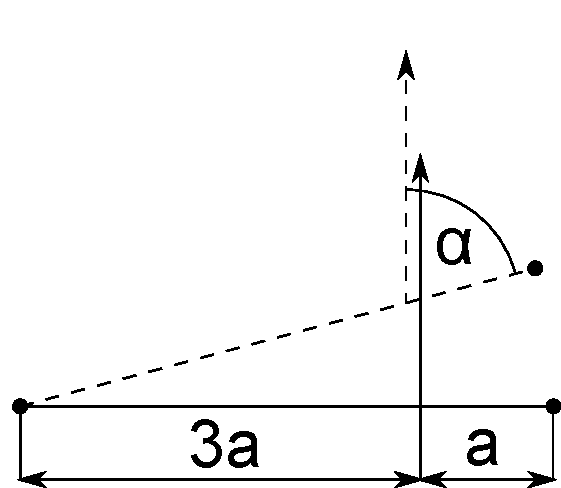
\includegraphics[width=0.23\textwidth]{2015-v3g-09-hantel}%
\vspace{-15 pt}%
\end{wrapfigure}
Horisontaalpinnal lebab hantel, mis koosneb kaalutust vardast pikkusega $l=4a$ ning selle otstele kinnitatud kahest ühesuguse massi ja hõõrdeteguriga väikesest klotsist. Varda külge kaugusele $a$ ühest klotsist on seotud pikk niit. Algul on niidi suund horisontaalne ja risti vardaga. Niiti aeglaselt tõmmates hakkab hantel pöörduma, sest alguses nihkub vaid üks klots. Milline on nurk $\alpha$ varda ja niidi vahel siis, kui ka teine klots nihkuma hakkab?

\fi


\ifHint
Pulgale mõjuvad kolm jõudu. Kuna niiti tõmmatakse aeglaselt, võib eeldada, et süsteemis kehtib nii jõudude kui ka jõumomentide tasakaal. Jõumomentide tasakaalu tõttu peavad jõudude rakendussirged lõikuma ühes punktis.
\fi


\ifSolution
Pulgale mõjuvad kolm jõudu. Jõumomentide tasakaalu tõttu peavad nende jõudude rakendussirged lõikuma ühes punktis, olgu see punkt $C$. Olgu niidi rakenduspunkt $N$ ja pulga otspunktid $A$ ning $B$, vt joonis. Kuna enne klotsi $A$ paigalt nihkumist pöörleb pulk ümber selle, siis punkti $B$ kiirusvektor on risti $AB$-ga, sama kehtib puntki $B$ rakendatud hõõrdejõu vektori jaoks; sestap $\angle ABC=\frac{\pi}{2}$. Et nihkuma hakkamise hetkel on hõõrdejõud võrdsed, siis jõudude kolmnurk $\vec F_1+\vec F_2=\vec T$ on võrdhaarne, järelikult on võrdhaarne ka jõudude kolmnurgaga sarnane kolmnurk $CBE$ (sirge $BE$ on tõmmatud paralleelsena $\vec T$-ga ja $E$ asub $\vec F_1$ rakendussirgel, vt joonis).
Olgu $|CB|=b$; siis ka $|CE|=b$. Seetõttu kolmnurkade $ANC$ ja $ABE$ sarnasuse põhjal $|AC|=3b$. Pythagorase
teoreemist kolmnurga $ABC$ jaoks $9b^2=b^2+16a^2$, st $b=\sqrt 2a$. Seetõttu otsitav nurk 
\[
\angle BNC=\arctan \frac ba =\arctan \sqrt 2\approx\SI{0.96}{rad}\approx 55^\circ.
\]
\begin{center}
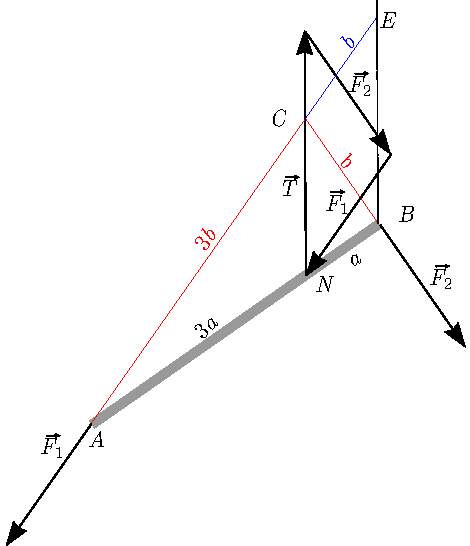
\includegraphics[width=0.7\textwidth]{2015-v3g-09-pulk_lah}
\end{center}
\fi


\ifEngStatement
% Problem name: Dumbbell with a thread
\begin{wrapfigure}{r}{0.23\textwidth}%
\vspace{-5 pt}%
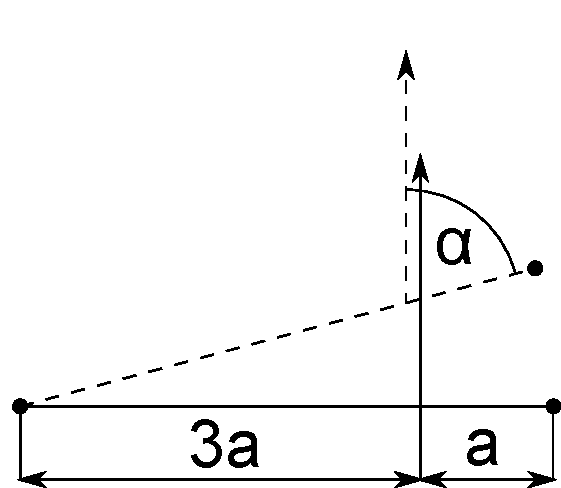
\includegraphics[width=0.23\textwidth]{2015-v3g-09-hantel}%
\vspace{-15 pt}%
\end{wrapfigure}
A dumbbell is lying on a horizontal ground. The dumbbell consists of a weightless rod of length $l=4a$ and two small blocks with identical masses and coefficients of friction that are attached to the ends of the rod. A long thread is tied to the rod at a length $a$ from one of the blocks. Initially the direction of the thread is horizontal and perpendicular to the rod. When the thread is slowly pulled the dumbbell starts to turn because at first only one block is being shifted. What is the angle $\alpha$ between the rod and the thread when the other block also starts to shift?
\fi


\ifEngHint
Three forces are applied to the rod. Because the thread is pulled at slowly you can assume that both the force and torque balance are applied in the system. Because of the torque balance the extensions of the forces have to intersect at one point.
\fi


\ifEngSolution
Three forces are applied to the rod. Due to the torque balance the extensions of these forces have to intersect at one point, let this point be $C$. Let the thread’s application point be $N$ and the ends of the rod $A$ and $B$, see figure. Because the rod is rotating around the block $A$ before it starts to shift then the point’s $B$ velocity vector is perpendicular to $AB$ and the friction’s vector is applied to the point $B$; because of this $\angle ABC=\frac{\pi}{2}$. Because at the moment of the displacement’s start the frictions are equal then the force triangle $\vec F_1+\vec F_2=\vec T$ is an isosceles triangle, therefore the similar triangle $CBE$ of the force triangle is also an isosceles triangle (the line $BE$ is drawn in parallel to $\vec T$ and $E$ is located on the extension of $\vec F_1$, see figure). Let $|CB|=b$; then also $|CE|=b$. Then due to the similarity of the triangles $ANC$ and $ABE$ we can see that $|AC|=3b$. From the Pythagorean theorem for the triangle $ABC$ we get $9b^2=b^2+16a^2$, meaning $b=\sqrt 2a$. Because of this the desired angle $\angle BNC=\arctan \frac ba =\arctan \sqrt 2\approx\SI{0.96}{rad}\approx 55^\circ$
\begin{center}
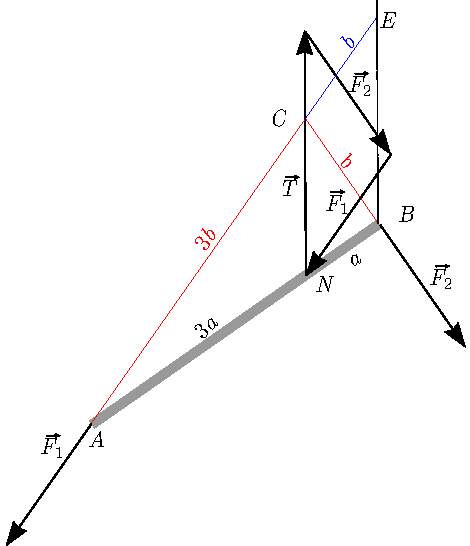
\includegraphics[width=0.7\textwidth]{2015-v3g-09-pulk_lah}
\end{center}
\fi
}